% Chapter Template

\chapter{Goal Management} % Main chapter title

\label{chapter:goal_management} % Change X to a consecutive number; for referencing this chapter elsewhere, use \ref{ChapterX}

\lhead{Chapter . \emph{Goal Management}} % Change X to a consecutive number; this is for the header on each page - perhaps a shortened title
In this Chapter we introduce the goal management characteristics of our system. Section \ref{sec:goal_management-intro} introduces the important topic of goal generation and management. Section \ref{sec:goal_management-overview} shows the main characteristics of this layer. Finally, section \ref{sec:goal_management-choosing} discusses in details the characteristics of our implementation.

\section{Introduction}
\label{sec:goal_management-intro}
An essential characteristic of an intelligent robot is acting with goal-oriented behaviors. Managing and generating goals has not been a primary focus of the AI community and, to our knowledge, there are not many works that deal with this important, and complex, subject. 

Let's imagine, for example, an household robot, helping a family to accomplish a number of task. At each moment, this robot can have several different goals, which could pre-programmed, requested by users, or selected by the robot by reasoning on the state of the world. New goals could even arise while the robot is already acting. What should the robot do in these situations? Should it abandon the current task and start executing a more important one? Or perhaps, if the current task is almost accomplished, should it finish executing it?  

It's clear that managing goals is a hard problem, involving issues such as scheduling and risk analysis. An example of work that studies this issues is \cite{hanheide2010framework}, where the authors present a framework to generate and manage goals in a robotic system. Goals are generated based on the system's state from a number of generators, and encoded in terms of importance and urgency. The framework has been used in a robotic explorer architecture.

\section{Overview}
\label{sec:goal_management-overview}
While goal management is not a focus in this work, we introduce a simple system that allows the robot to select which goal to activate from a list of possible goals. This layer is able to:

\begin{itemize}
\item Generate new goals by reasoning on the current state of the world.
\item Select the next goal to achieve by analyzing the importance of each possible goal.
\item Activate other layers of the system to achieve goals.
\item Managing goals by pausing the current goal, aborting it, switch from one goal to another, etc.
\end{itemize}


We do not include mechanisms for scheduling or to evaluate the length of time to achieve a goal, which would improve the quality of choices performed by this layer .

\section{Generating and Choosing Goals}
\label{sec:goal_management-choosing}
This layer possesses a list of possible goals that can be achieved by the robot, which may differ from the list of intentions introduced in section \ref{sec:situation_assessment-intention_recognition}, since some goals could be achieved only by humans or only by the robot. At each moment, the layer also has a list of instantiated goals, that need to be managed.

Each goal is represented by a tuple $(name, parameters, activation, priority, status$), where $name$ is a unique string identifying the goal, $parameters$ is a set of variables related to a specific instance of a goal, $activation$ is a set of properties used to generate an instance of the goal, and $priority$ is a string that can assume the possible values $(low, medium, high)$ and represents the importance of the goal. The priority of a task is precomputed, or can be selected by the human when requesting a task. At each moment a goal instance has a $status$, which can be $active$, meaning that the robot is executing actions to achieve it; $ready$, meaning that the goal can be selected to become $active$; $paused$, meaning that the goal was $active$ but has been temporarily abandoned to pursue another goal; or $aborted$, meaning this instance of the goal can be erased.  

At the start of the system, there are no active goals. Goals can be instantiated, starting with $ready$ status, in different ways:
\begin{itemize}
\item The $activation$ list of the goal becomes true in the Situation Assessment Database. This feature can be used to program the robot to perform goals in specific circumstances. For example the robot could select a goal to clean the living room table after launch, if there are dishes on it.
\item There is a request from the human to perform a goal. 
\item There is a request the Situation Assessment Layer to warn a human (see \ref{subsec:situation_assessment-proactive_behaviors}).
\item The robot detects a new human intention. If there is a corresponding goal in this layer the robot will create a new instance of it. 
\end{itemize}


\begin{figure}[h!]
	\centering
	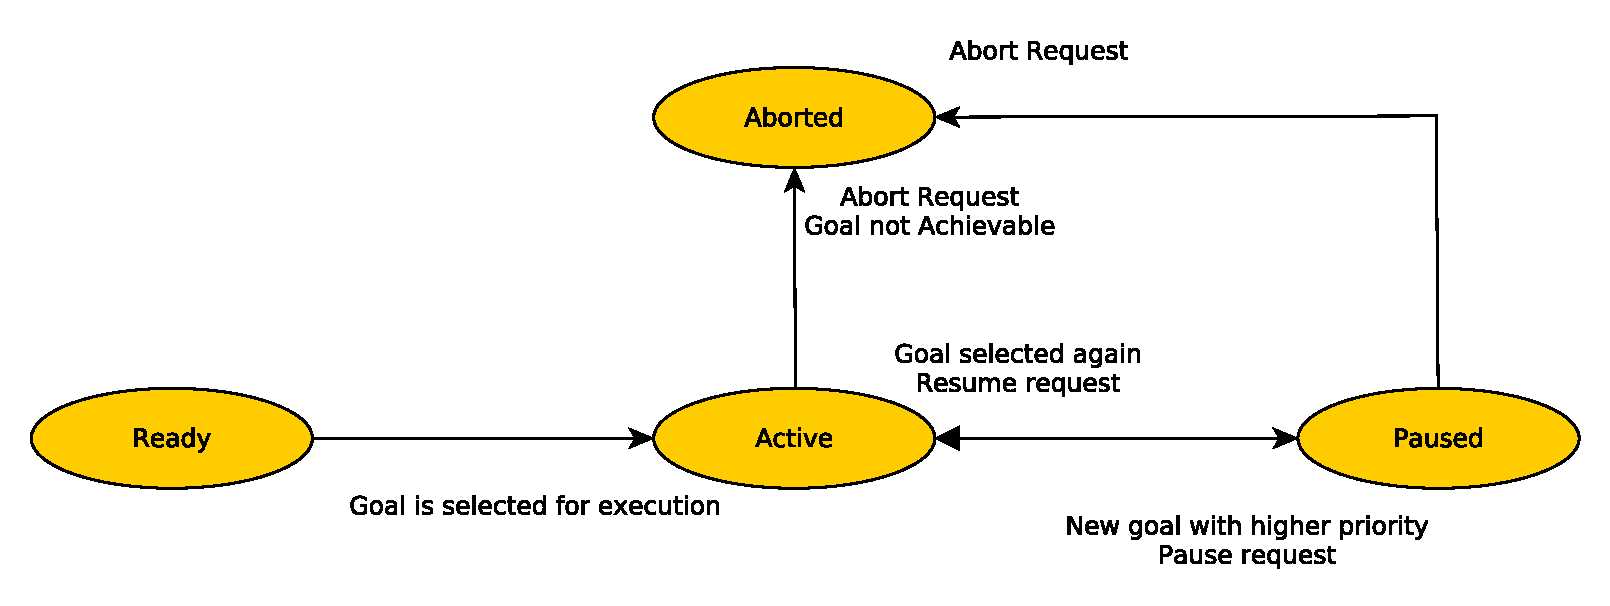
\includegraphics[clip,scale=0.6]{img/goal_management/goal_cycle.pdf}
	\caption{The state machine representing transitions between the statuses of a goal.}
	\label{fig:goal_management-goal_cycle}
\end{figure}



The robot will select a $ready$ goal to become $active$. The $active$ goal is selected by choosing the goal with the highest priority, with random selection used to solve conflicts.

If the robot is executing a plan to achieve a goal, and new goal with a higher $priority$ becomes $ready$, the current goal becomes $paused$, and the robot considers $active$ thje new goal. A goal can also become $not active$ if it was $active$ and there is no plan to achieve it, if it has been achieved, or if the human requests the robot to abort it.

When a goal is selected as active, the robot will contact the Plan PRoduction and Management layer to achieve it, as explained in chapter \ref{chapter:plan_management}



